% --------------------------------------------------------------
% This is all preamble stuff that you don't have to worry about.
% Head down to where it says "Start here"
% --------------------------------------------------------------

\documentclass[12pt]{article}
\usepackage[margin=0.75in]{geometry}
\usepackage{amsmath,amsthm,amssymb,mathtools,graphicx,enumitem,hyperref,hyphenat,float}
% \usepackage[paperwidth=\maxdimen,paperheight=\maxdimen]{geometry}
\usepackage{svg}
\usepackage{register}
\usepackage{rotating}
\DeclarePairedDelimiter{\ceil}{\lceil}{\rceil}
\newcommand{\N}{\mathbb{N}}
\newcommand{\Z}{\mathbb{Z}}
\newcommand{\Q}{\mathbb{Q}}
\newcommand{\R}{\mathbb{R}}
\newcommand{\F}{\mathbb{F}}
\newcommand{\C}{\mathbb{C}}
\newcommand{\lub}{\mathrm{lub}}
\newcommand{\g}{\mathrm{glb}}
\newcommand{\seq}{\subseteq}
\newcommand{\e}{\epsilon} 
\newcommand{\de}{\delta}
\newcommand{\mbf}{\mathbf}
\newcommand{\es}{\emptyset}
\newcommand{\mc}{\mathcal}
\newcommand{\un}{\cup}
\newcommand{\ic}{\cap}
\newcommand{\gen}[1]{\ensuremath{\langle #1\rangle}}
\newcommand{\spn}{\mathrm{span \ }}
\newcommand{\dm}{\mathrm{dim \ }}
\newcommand{\Lm}{\mathcal{L}}
\newcommand{\nll}{\mathrm{null \ }}
\newcommand{\rng}{\mathrm{range \ }}
\newcommand{\dgr}{\mathrm{deg \ }}
\newcommand{\Lim}{\lim\limits}
\newcommand{\Sum}{\sum\limits}
\newcommand{\Pt}{\|P\|}
\newcommand{\dmn}{\mathrm{dom \ }}
\newcommand{\Prod}{\prod\limits}
\DeclarePairedDelimiter\floor{\lfloor}{\rfloor}
\DeclarePairedDelimiter\ev{\langle}{\rangle}
\newcommand*\dif{\mathop{}\!\mathrm{d}}
\newcommand{\Beta}{\mathcal B}
\newcommand{\Seq}{\mathrm{Seq }}
\theoremstyle{plain}

\newtheorem{thm}{Theorem} % reset theorem numbering for each chapter
\newtheorem{lem}{Lemma}
\newtheorem{cor}{Corollary}
\newtheorem{rem}{Remark}
\newtheorem{fct}{Fact}
\newtheorem{cnj}{Conjecture}
\newtheorem{asm}{Assumption}
\theoremstyle{definition}
\newtheorem{defn}{Definition}
\newtheorem{exmp}{Example} % same for example numbers
\renewcommand{\regBitWidth}{16}
	
\begin{document}
	
% --------------------------------------------------------------
%                         Start here
% --------------------------------------------------------------
	
\begin{titlepage}

	\newcommand{\HRule}{\rule{\linewidth}{0.5mm}} % Defines a new command for the horizontal lines, change thickness here
	
	\center % Center everything on the page
	 
	%----------------------------------------------------------------------------------------
	%	HEADING SECTIONS
	%----------------------------------------------------------------------------------------
	
	\textsc{\LARGE Faculty of Engineering, Cairo University}\\[0.5cm] % Name of your university/college
	\textsc{\large Computer Engineering Department}\\[1.5cm] % Minor heading such as course title
	
	\textsc{\Large Computer Architecture Course Project}\\[0.5cm] % Major heading such as course name
	
	%----------------------------------------------------------------------------------------
	%	TITLE SECTION
	%----------------------------------------------------------------------------------------
	
	\HRule \\[0.4cm]
	{ \huge \bfseries Orthrus - Phase 1 Report}\\[0.4cm] % Title of your doc
	\HRule \\[1.5cm]
	 
	%----------------------------------------------------------------------------------------
	%	AUTHOR SECTION
	%----------------------------------------------------------------------------------------
	
	\begin{minipage}{0.4\textwidth}
	\begin{flushleft} \large
	Ahmad Khaled \\
	Maryam Shalaby \\
	Zeinab Rabie \\
	Omnia Zakaria
	\end{flushleft}
	\end{minipage}
	\begin{minipage}{0.4\textwidth}
	\begin{flushright}\large
        Section 1 BN. 03 \\
        Section 2 BN. 21 \\
        Section 1 BN. 22 \\
        Section 1 BN. 23 \\
	\end{flushright}
	\end{minipage}\\[1cm]
	
	% If you don't want a supervisor, uncomment the two lines below and remove the section above
	%\Large \emph{Author:}\\
	%John \textsc{Smith}\\[3cm] % Your name
	
	%----------------------------------------------------------------------------------------
	%	LOGO SECTION
	%----------------------------------------------------------------------------------------
	
	
\includegraphics[scale=0.15]{cu_logo.png}\\[1cm] % Include a department/university logo - this will require the graphicx package
	 
	%----------------------------------------------------------------------------------------
	
	\vfill % Fill the rest of the page with whitespace
	
\end{titlepage}

\section{Introduction}
Orthrus is a pipelined static dual-issue microprocessor implementing a RISC ISA similar to the MIPS ISA. In the following sections we outline the instruction format, the general design of the processor, as well as the pipeline stages design.

\section{Instruction Set Architecture}
    The structure for the IR for two-operand instructions is given in Figure~\ref{IR-TwoOp}. The structure for one-operand instructions is given in Figure~\ref{IR-SingleOp}. The structure for branching instructions is given in Figure~\ref{IR-Branch}. The structure for the rest of the instructions is given in Figure~\ref{IR-Misc}.
    \begin{table}[H]
        \centering
        \begin{tabular}{c|c|c|c|c|}
            \cline{2-5}
            \textbf{Direct}   & Register & Auto-increment & Auto-decrement & Indexed \\ \cline{2-5} 
            \textit{Code}     & 000      & 001            & 010            & 011     \\ \cline{2-5} 
            \textbf{Indirect} & Register & Auto-increment & Auto-decrement & Indexed \\ \cline{2-5} 
            \textit{Code}     & 100      & 101            & 110            & 111     \\ \cline{2-5} 
        \end{tabular}
        \caption{Addressing Mode Codes}
        \label{addr-mode-codes}
    \end{table}
    \begin{table}[H]
        \centering
        \begin{tabular}{c|c|c|c|c|}
            \cline{2-5}
                            & $R_0$ & $R_1$ & $R_2$ & $R_3$ \\ \cline{2-5} 
            \textit{Code}   & 000      & 001            & 010            & 011     \\ \cline{2-5} 
                            & $R_4$ & $R_5$ & $R_6?$ & $R_7$ \\ \cline{2-5} 
            \textit{Code}   & 100      & 101            & 110            & 111     \\ \cline{2-5} 
        \end{tabular}
        \caption{Register Addressing Codes}
        \label{reg-addr-codes}
    \end{table}
    \begin{table}[H]
        \centering
        \begin{tabular}{|c|c|c|c|c|c|c|c|c|c|}
        \hline
        Instruction & MOV  & ADD  & ADC  & SUB  & SBC  & AND  & OR   & XNOR & CMP  \\ \hline
        OP Code     & 1111 & 1110 & 1101 & 1100 & 1011 & 1010 & 1001 & 1000 & 0111 \\ \hline
        \end{tabular}
        \caption{Two-Operand Instruction Codes}
        \label{two-operand-op-codes}
    \end{table}
    \begin{figure}[H]
        \centering
        \caption{IR Structure For Two-Operand Instructions}
        \label{IR-TwoOp}
        \vspace{0.5 cm}
        \regfield{}{4}{12}{{Instruction}}
        \regfield{}{3}{9}{{Source Address}}
        \regfield{}{3}{6}{{Source Register}}
        \regfield{}{3}{3}{{Destination Address}}
        \regfield{}{3}{0}{{Destination Register}} \\
        \vspace{0.5 cm}
        \begin{regdesc}\begin{reglist}
            \item [Instruction] specifies the instruction to execute. Possible codes given in Table~\ref{two-operand-op-codes}.
            \item [Source Address] specifies the addressing mode to choose for the source. Possible codes given in Table ~\ref{addr-mode-codes}.
            \item [Source Register] specifies the source register. Possible codes given in Table~\ref{reg-addr-codes}.
            \item [Destination Address] specifies the addressing mode to choose for the destination. Possible codes given in Table~\ref{addr-mode-codes}.
            \item [Destination Register] specifies the destination register. Possible codes given in Table~\ref{reg-addr-codes}.
        \end{reglist}\end{regdesc}
    \end{figure}
    \begin{table}[H]
        \centering
        \begin{tabular}{|c|c|c|c|c|c|c|c|c|c|c|c|}
            \hline
            Instruction & INC  & DEC  & CLR  & INV  & LSR  & ROR  & RRC  & ASR & LSL & ROL & RLC  \\ \hline
            OP Code     & 0000 & 0001 & 0010 & 0011 & 0100 & 0101 & 0110 & 0111 & 1000 & 1001 & 1010 \\ \hline
        \end{tabular}
        \caption{Single Operand Instruction Codes}
        \label{single-operand-op-codes}
    \end{table}
    \begin{figure}[H]
        \centering
        \caption{IR Structure For Single-Operand Instructions}
        \label{IR-SingleOp}
        \vspace{0.5 cm}
        \regfield{}{4}{12}{0110}
        \regfield{}{4}{8}{{Instruction}}
        \regfield{}{2}{6}{00}
        \regfield{}{3}{3}{{Operand Address}}
        \regfield{}{3}{0}{{Operand Register}} \\
        \vspace{0.5 cm}
        \begin{regdesc}\begin{reglist}            
            \item [Instruction] specifies the instruction to execute. Possible codes given in Table~\ref{single-operand-op-codes}.
            \item [Operand Address] specifies the addressing mode to choose for the operand. Possible codes given in Table~\ref{addr-mode-codes}.
            \item [Operand Register] specifies the operand register. Possible codes given in Table~\ref{reg-addr-codes}.
        \end{reglist}\end{regdesc}
    \end{figure}
    \begin{table}[H]
        \centering
        \begin{tabular}{|c|c|c|c|c|c|c|c|}
            \hline
            Instruction & BR  & BEQ  & BNE  & BLO  & BLS  & BHI  & BHS \\ \hline
            OP Code     & 000 & 001 & 010 & 011 & 100 & 101 & 110 \\ \hline
        \end{tabular}
        \caption{Branching Instruction Codes}
        \label{br-op-codes}
    \end{table}
    \begin{figure}[H]
        \centering
        \caption{IR Structure For Branching Instructions}
        \label{IR-Branch}
        \vspace{0.5 cm}
        \regfield{}{4}{12}{0101}
        \regfield{}{3}{9}{{Instruction}}
        \regfield{}{9}{0}{{Operand}} \\
        \vspace{0.5 cm}
        \begin{regdesc}\begin{reglist}            
            \item [Instruction] specifies the instruction to execute. Possible codes given in Table~\ref{br-op-codes}.
            \item [Operand] specifies the branching offset.
        \end{reglist}\end{regdesc}
    \end{figure}
    \begin{table}[H]
        \centering
        \begin{tabular}{|c|c|c|c|c|c|c|}
            \hline
            Instruction & JSR  & RTS  & HITR  & IRET  & HLT  & NOP  \\ \hline
            OP Code     & 0100 & 0011 & 0011 & 0010 & 0001 & 0000 \\ \hline
        \end{tabular}
        \caption{Miscellaneous Instruction Codes}
        \label{misc-op-codes}
    \end{table}
    \begin{figure}[H]
        \centering
        \caption{IR Structure For Miscellaneous Instructions}
        \label{IR-Misc}
        \vspace{0.5 cm}
        \regfield{}{4}{12}{{Instruction}}
        \regfield{}{1}{11}{{Extra}}
        \regfield{}{11}{0}{{Operand}} \\
        \vspace{0.5 cm}
        \begin{regdesc}\begin{reglist}            
            \item [Instruction] specifies the instruction to execute (except for differentiating RTS and HITR, done using Extra bit). Possible codes given in Table~\ref{misc-op-codes}.
            \item [Extra] useful for JSR and HITR only. specifies whether the Operand is given directly or using a register/addressing mode for JSR. Indicates HITR when instruction is $0011$ and Extra$=1$, indicates RTS if instruction is $0011$ and Extra$=0$. 
            \item [Operand] useful for JSR only. specifies the memory location to jump  to.
        \end{reglist}\end{regdesc}
    \end{figure}
\pagebreak

\section{Schematics}
    Figures~\ref{sys-schematic-1} and ~\ref{sys-schematic-2} include the schematic for the design.
    \pagebreak
    \begin{sidewaysfigure}[h]
        \centering
        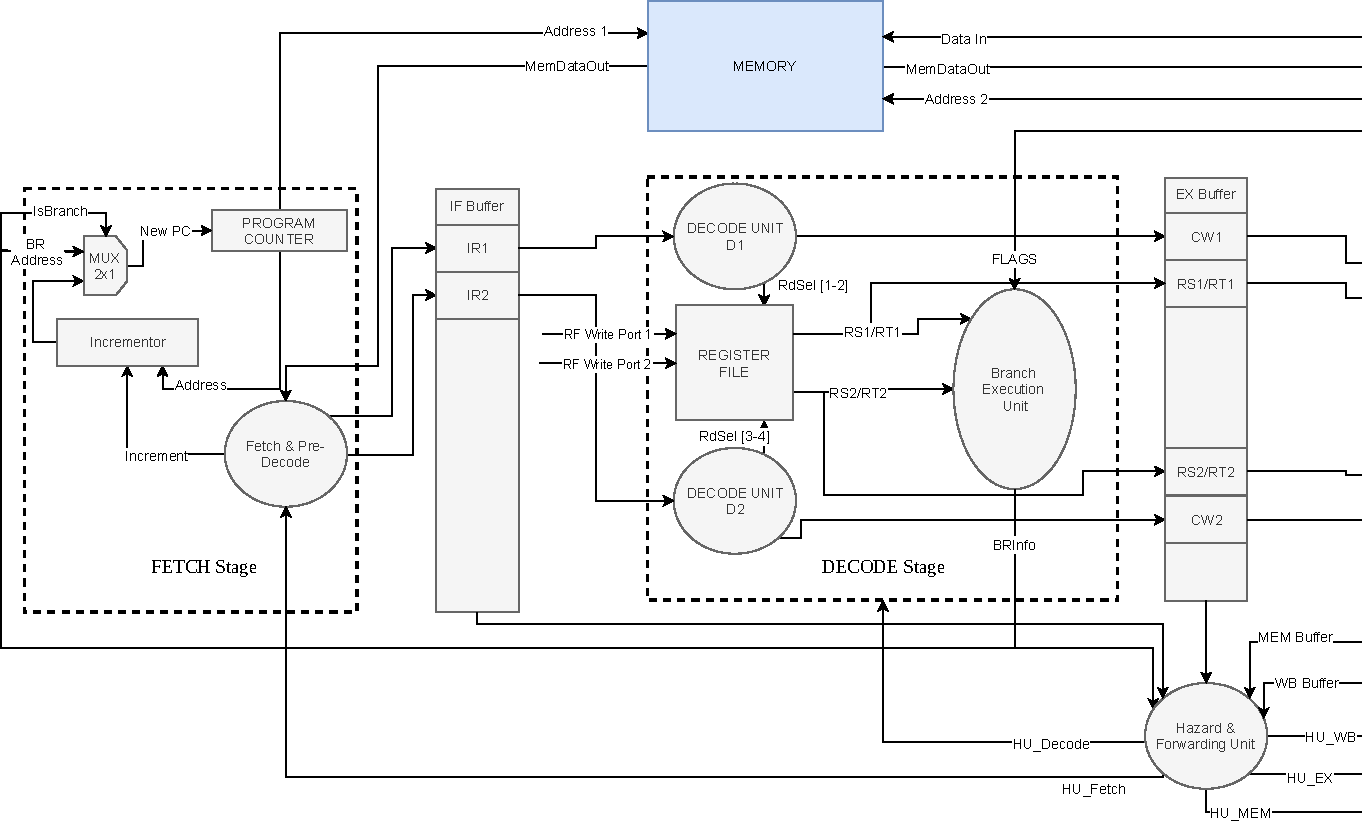
\includegraphics[page=1]{Diagrams/SystemOverviewSplit}
        \caption{Overall Schematic Part 1}
        \label{sys-schematic-1}
    \end{sidewaysfigure}
    \begin{sidewaysfigure}[h]
        \centering
        \includegraphics[page=2]{Diagrams/SystemOverviewSplit}
        \caption{Overall Schematic Part 2}
        \label{sys-schematic-2}
    \end{sidewaysfigure}
    % \include{OverviewFig}
\pagebreak

\section{Pipeline}
\subsection{Stages}
\subsection{Hazards}


% --------------------------------------------------------------
%     You don't have to mess with anything below this line.
% --------------------------------------------------------------
			
\end{document}	